\section{Funciones Complejas}
    
Todas las funciones elementales de variables reales pueden ser extendidas al plano complejo, con solo cambiar la variable real $x$ por una variable compleja $z$.

\subsection[short]{Condiciones de Cauchy-Riemann}

    Partiendo de una función de variable compleja estable $f(z)$, se define su derivada tal cual como una función real.

    \begin{equation*}
        \lim_{\delta z \rightarrow 0} \frac{f(z + \delta z) - f(\delta z)}{z + \delta z - z} = \frac{\delta f}{\delta z} = \frac{df}{dz}
    \end{equation*}
    siempre que el limite sea \textbf{independiente} a la aproximación particular al punto $z$, es decir, que para que el límite exista las aproximaciones con $\delta y = 0$  y $delta x = 0$  deben ser iguales. Eso es debido a que en una función compleja hay dos formas en las que podemos aproximarnos a un limites (tal como lo muestra la Fig.\ref*{fig:ich})

    \begin{figure}[h]
        \centering
        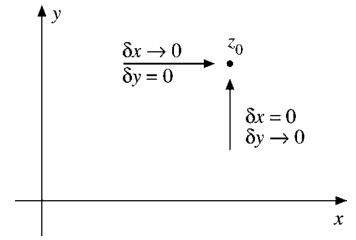
\includegraphics[width=0.4\textwidth]{imgs/ich.png}
        \caption{}
        \label{fig:ich}
    \end{figure}
    Considerando incrementos en $x$ y en $y$ entonces, 

    \begin{gather*}
        \delta z = \delta x + i\delta y\\
    \end{gather*}

    Ahora, teniendo en cuenta que $f  = u(x,y) + iv(x,y)$ entonces 
    \begin{gather*}
        \delta f = \delta u + i \delta v
    \end{gather*}

    por tanto,

    \begin{equation*}
        \frac{\delta f}{\delta z} = \frac{\delta u + i\delta v}{\delta x + i\delta y}
    \end{equation*}
    
    Realizando la aproximación al limite cuando $\delta y = 0$ y $\delta x \rightarrow 0$

    \begin{equation*}
        \lim_{\delta z \rightarrow 0}  \frac{\delta f}{\delta z} = \lim_{\delta x \rightarrow 0} \left(\frac{\delta u}{\delta x}+ i\frac{ \delta v}{\delta x}\right) = \frac{\partial u}{\partial x} + i \frac{\partial v}{\partial x}
    \end{equation*}
    para cuando $\delta x = 0$ y $\delta y \rightarrow 0$ 
    \begin{equation*}
        \lim_{\delta z \rightarrow 0}  \frac{\delta f}{\delta z} = \lim_{\delta y \rightarrow 0} \left(\frac{\delta u}{i\delta y}+ \frac{ \delta v}{\delta y}\right) = - i\frac{\partial u}{\partial y} + \frac{\partial v}{\partial y}
    \end{equation*}
    entonces para que el limite exista se debe cumplir

    \begin{gather*}
        \lim_{\delta x \rightarrow 0} \left(\frac{\delta u}{\delta x}+ i\frac{ \delta v}{\delta x}\right) = \lim_{\delta y \rightarrow 0} \left(\frac{\delta u}{i\delta y}+ \frac{ \delta v}{\delta y}\right)\\
        \frac{\partial u}{\partial x} + i \frac{\partial v}{\partial x} = - i\frac{\partial u}{\partial y} + \frac{\partial v}{\partial y}
    \end{gather*}
    ahora como $\Im$ y $\Re$ son linealmente independientes entonces 

    \begin{align*}
        \frac{\partial u}{\partial x} =  \frac{\partial v}{\partial y} && \frac{\partial v}{\partial x} = - \frac{\partial u}{\partial y}
    \end{align*}
    estas son las \textit{condiciones de Cauchy-Riemann} y se tienen que cumplir para que la derivada de una función compleja exista, ahora cambiando un poco la notación se establece que

    \begin{gather*}
        \frac{\partial u}{\partial x} =  \frac{\partial v}{\partial y}  \longrightarrow  U_x = V_y\\
        \frac{\partial v}{\partial x} =  -\frac{\partial u}{\partial y}  \longrightarrow  V_x = -U_y\\
    \end{gather*}

    Para una función de variable compleja que cumpla con las condiciones de Cauchy-Riemann y las derivadas parciales sobre $u(x,y)$ y $v(x,y)$ son continuas entonces se puede escribir

    \begin{gather*}
        \frac{\delta f}{\delta z} = \frac{(U_x + iV_x)\delta x + (U_y + iV_y)\delta y}{\delta x + i\delta y}
    \end{gather*}

    



